\documentclass[11pt]{article}
\usepackage[a4paper,margin=2.6cm]{geometry}
\usepackage{amsmath,amssymb,amsthm}
\usepackage{graphicx}
\usepackage{booktabs}
\usepackage{xcolor}
\usepackage[colorlinks=true,linkcolor=blue!50!black,citecolor=blue!50!black]{hyperref}
\usepackage{microtype}

\graphicspath{{figs/}}

\newtheorem{observation}{Observation}
\newtheorem{conjecture}{Conjecture}
\newtheorem{lemma}{Lemma}
\newcommand{\dd}{\,\mathrm{d}}

\title{Melting kinks: a sweeping-curvature mechanism for logarithmic growth\\
in a coupled monotone--convex variational problem}
\author{}
\date{July 2026}

\begin{document}
\maketitle

\begin{abstract}
We study the variational problem of maximizing
$J[f,g]=\int_0^1\!\!\int_{-1}^{1} f_t\,g_{xx}\dd x\dd t$ over pairs of
time-monotone, $x$-convex, Lipschitz functions with zero boundary and
terminal/initial conditions. Single-kink (tent) competitors provably cap at
$J=2$. Numerical mesh optimization reaches a certified $J=3.055$, strictly
breaching the tent cap, and the optimizers share a common structure we call
\emph{melting}: the curvature of each profile, a single Dirac point mass in
the tent regime, spreads into a finite-width band that drifts across the
domain, harvesting the rise budget of every location it visits. The gain per
dyadic refinement level is nearly constant ($\approx 0.215$ per octave over
the two clean octaves affordable), the signature of logarithmic growth
$J\sim c\log_2 N_x$ and hence of an unbounded supremum. We describe the
mechanism, give a scaling analysis showing that \emph{strictly} self-similar
cascades are necessarily bounded while an \emph{anisotropic} cascade
(widths, lifetimes and rise-shares contracting; travel length fixed) yields
a constant per-generation gain, and formulate a renormalization
cell problem whose fixed point would decide the dichotomy --- boundedness
versus logarithmic blow-up --- by induction rather than extrapolation.
\end{abstract}

\section{The problem}

Let $Q=[-1,1]\times[0,1]$ with coordinates $(x,t)$. We seek
\begin{equation}
\label{eq:J}
\sup\; J[f,g]\;=\;\sup\int_0^1\!\!\int_{-1}^{1} f_t(x,t)\,g_{xx}(x,t)\dd x\dd t
\end{equation}
over pairs $f,g:Q\to\mathbb{R}$ subject to
\begin{align*}
&\text{convexity in }x:\quad f(\cdot,t),\,g(\cdot,t)\ \text{convex for all }t;\\
&\text{Lipschitz bound:}\quad |f_x|\le 1,\ |g_x|\le 1;\\
&\text{monotonicity:}\quad f_t\ge 0,\quad g_t\le 0;\\
&\text{boundary:}\quad f(\pm1,t)=g(\pm1,t)=0;\qquad
\text{ends:}\quad f(x,1)=0,\ g(x,0)=0.
\end{align*}
Thus $f\le 0$ rises monotonically to zero and $g\le 0$ decays monotonically
from zero; both are convex ``dents'' at every time. Since $g(\cdot,t)$ is
convex and piecewise linear in the discrete setting, $g_{xx}$ is a
nonnegative measure in $x$ (a sum of point masses at the kinks of $g$), and
the integral \eqref{eq:J} is well defined as a harvest of $f$'s rise sampled
along $g$'s kinks.

Two budget identities control everything that follows.
\emph{Rise budget:} for each $x$,
\begin{equation}
\label{eq:rise}
\int_0^1 f_t(x,t)\dd t \;=\; -f(x,0)\;\le\; 1-|x|,
\end{equation}
with equality on the right iff $f(\cdot,0)$ is the full tent
$-\,(1-|x|)$. \emph{Curvature budget:} for each $t$, the total curvature
mass of a slice is its total slope change, capped by the Lipschitz bound:
\begin{equation}
\label{eq:mass}
\int_{-1}^{1} g_{xx}(\cdot,t)\;=\;g_x(1^-,t)-g_x(-1^+,t)\;\le\;2 .
\end{equation}
No admissible motion creates curvature mass; it can only be
\emph{redistributed} in $x$ and $t$.

\begin{observation}[tent cap]
\label{obs:tent}
If $g(\cdot,t)$ keeps a single kink at a fixed location $x_0$ for all $t$
(the ``rigid tent''), then
$J=\int_0^1 m(t)\,f_t(x_0,t)\dd t \le 2\int_0^1 f_t(x_0,t)\dd t
\le 2\,(1-|x_0|)\le 2$, using \eqref{eq:mass} then \eqref{eq:rise}. The value
$J=2$ is attained by full-depth tents ($x_0=0$, both budgets saturated).
\end{observation}

Any $J>2$ therefore requires the curvature of $g$ to \emph{move}. The open
question we address is whether $\sup J<\infty$. A closely related quantity
is the peak-rise functional
\begin{equation}
\label{eq:H}
H[f]\;=\;\int_0^1 \sup_x f_t(x,t)\dd t ,
\end{equation}
which majorizes what any single unit of moving curvature mass can harvest
along its trajectory $p(t)$:
$\int_0^1 f_t(p(t),t)\dd t\le H[f]$. Growth of $\sup J$ and growth of
$\sup H$ are two faces of the same question.

\section{Numerical evidence: the tent cap is breached}

The problem was discretized on rectangular $N_x\times M_t$ grids and
maximized numerically, with the resulting fields certified feasible and the
objective re-evaluated independently. Table~\ref{tab:levels} and
Figure~\ref{fig:levels} summarize the refinement study; the best certified
value is
\[
J \;=\; 3.0553 \qquad (N_x=65,\ M_t=257),
\]
a strict breach of the tent cap by more than $50\%$.

\begin{table}[ht]
\centering
\caption{Certified objective per refinement level. Levels 1--6 refine time
alongside space; levels 7--8 refine space while starving time.}
\label{tab:levels}
\begin{tabular}{ccccl}
\toprule
level $k$ & $N_x=2^k{+}1$ & $M_t$ & $J$ & remark\\
\midrule
1--3 & 3--9 & 129 & 2.0000 & tent regime (cap attained)\\
4 & 17 & 129 & 2.6253 & first breach\\
5 & 33 & 129 & 2.8361 & $\Delta J=+0.211$\\
6 & 65 & 257 & 3.0553 & $\Delta J=+0.219$\\
\midrule
7 & 129 & 129 & 2.9788 & $t$-starved: $J$ \emph{decreases}\\
8 & 257 & 65 & 2.8450 & badly $t$-starved\\
\bottomrule
\end{tabular}
\end{table}

\begin{figure}[ht]
\centering
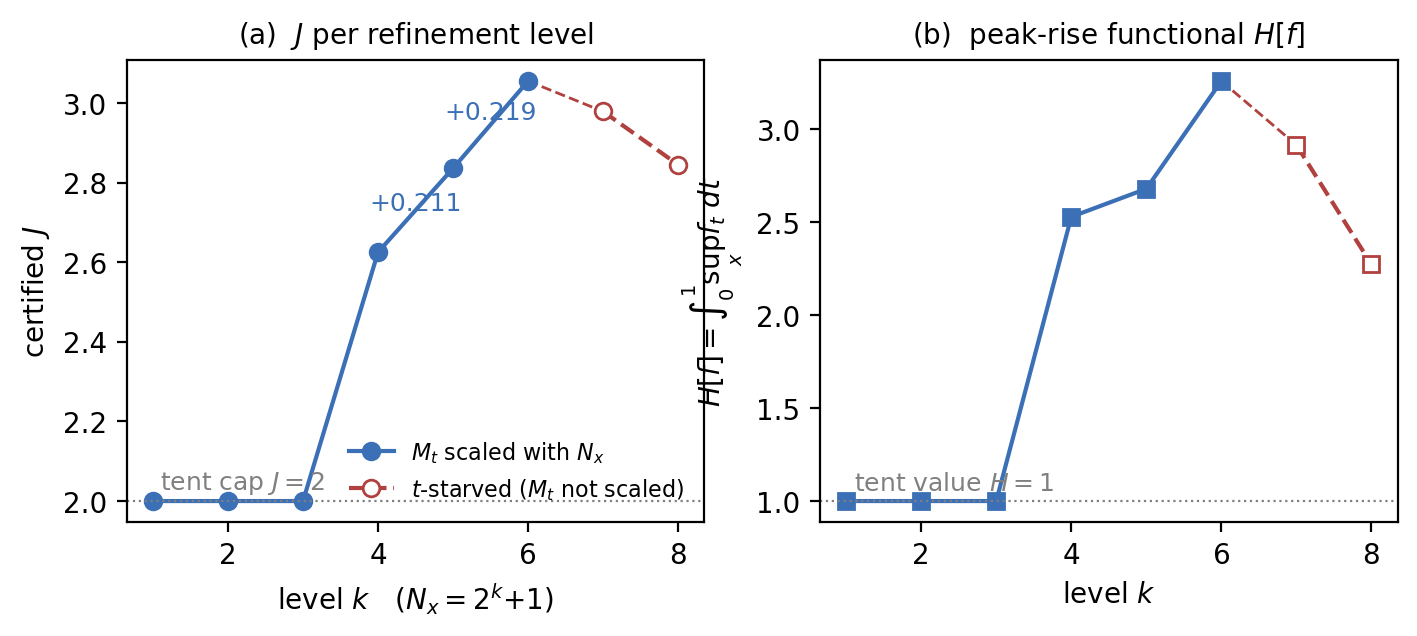
\includegraphics[width=\textwidth]{fig_levels.png}
\caption{(a) Certified $J$ per dyadic refinement level. Below $N_x=17$ the
optimizer sits exactly on the tent cap $J=2$; above it, each clean octave
(space \emph{and} time refined together, filled markers) adds a nearly
constant $\Delta J\approx 0.215$. Refining space while starving time (open
markers) moves $J$ \emph{backwards} --- resolution in $t$ is load-bearing.
(b) The peak-rise functional $H[f]$ of \eqref{eq:H} grows in step with $J$.}
\label{fig:levels}
\end{figure}

At every level, including the highest, the boundary slices are
\emph{exact} full-depth tents: $\min_x f(x,0)=\min_x g(x,1)=-1.0000$ with
apex at $x=0$. This is forced by \eqref{eq:rise} and its mirror for $g$: the
end slices are pure budget stock, and the optimum stocks them maximally. All
structure lives in the \emph{interior} slices.

\section{What the optimizer builds: melting}

\begin{figure}[ht]
\centering
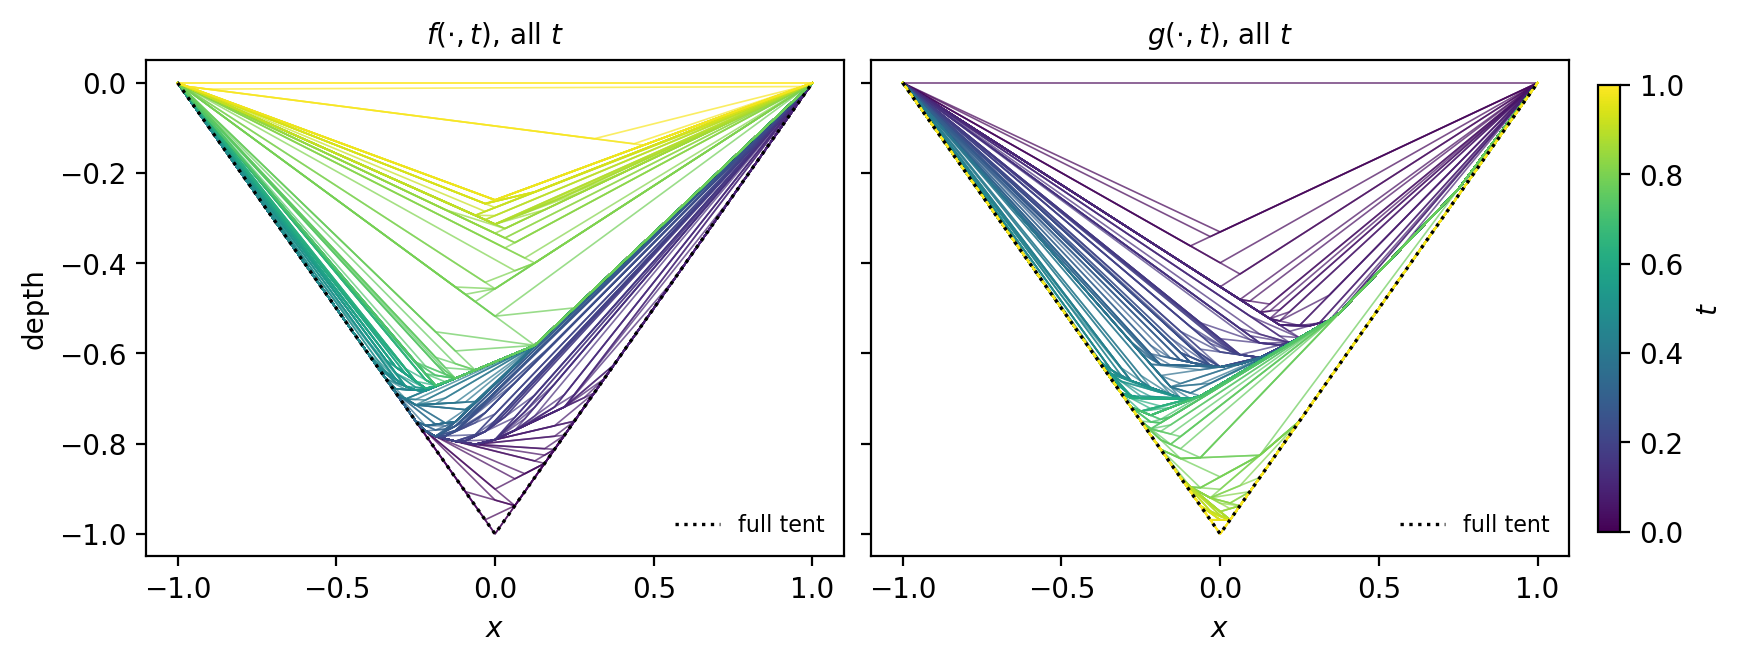
\includegraphics[width=\textwidth]{fig_slices.png}
\caption{\emph{Every} spatial slice of the certified $J=3.055$ solution, one
line per time node ($M_t=257$), colored by $t$. The full-depth end slices
($t=0$ for $f$, $t=1$ for $g$) sit exactly on the tent (dotted black); as
time advances each profile lifts toward zero while its basin bottom is
displaced from the center and migrates --- the melt. The Lipschitz-1 arms
are preserved at every $t$; only the vertex melts into a wide, moving,
rounded basin.}
\label{fig:slices}
\end{figure}

\begin{figure}[ht]
\centering
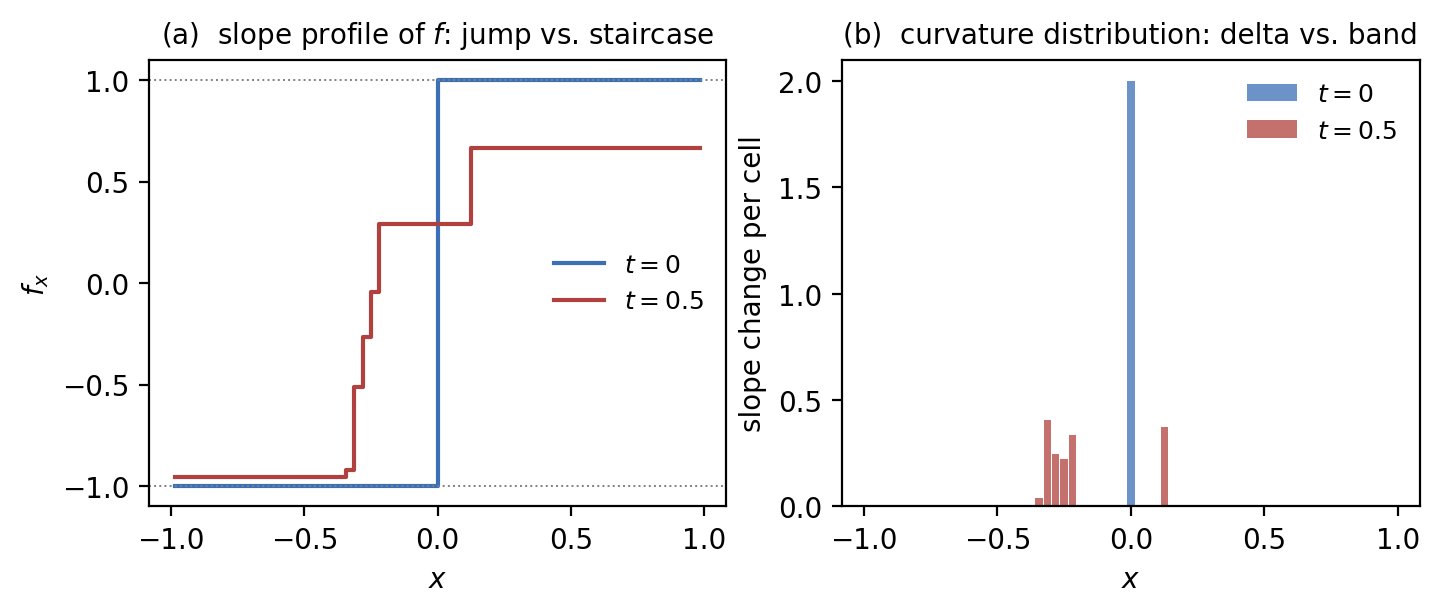
\includegraphics[width=\textwidth]{fig_slopes.png}
\caption{The same phenomenon in slope and curvature coordinates, for
$f(\cdot,t)$. (a) At $t=0$ the slope is a single $-1\to+1$ jump (a tent); at
$t=0.5$ it is a staircase climbing through an interval of width
$\approx0.5$. (b) The corresponding curvature distribution: a single cell
holding the full mass $2$ at $t=0$, versus the same ($\le2$) mass spread
over many cells at $t=0.5$ --- the largest single cell holds only $25\%$.
This spreading, together with the drift visible in
Figure~\ref{fig:melt}, is what we call \emph{melting}.}
\label{fig:slopes}
\end{figure}

Figure~\ref{fig:slices} shows spatial slices of the $J=3.055$ field, and
Figure~\ref{fig:slopes} the same data in slope/curvature coordinates. The
structure is consistent at every refinement level:

\begin{quote}
\textbf{Melting.} The tent's curvature --- a single Dirac point mass
carrying the full slope change $2$ --- spreads into a \emph{distributed
band} of finite width (width $\approx0.47$ at $t=0.5$; the largest single
cell holds $25\%$ of the mass), and this band \emph{drifts} in $x$ as $t$
advances. The straight Lipschitz-1 arms survive untouched; only the sharp
V-bottom becomes a wide, rounded, moving basin. Total curvature mass per
slice never exceeds the cap \eqref{eq:mass} (measured: $1.62$ at $t=0.5$,
$2.00$ at the ends). Melting redistributes; it creates nothing.
\end{quote}

\begin{figure}[ht]
\centering
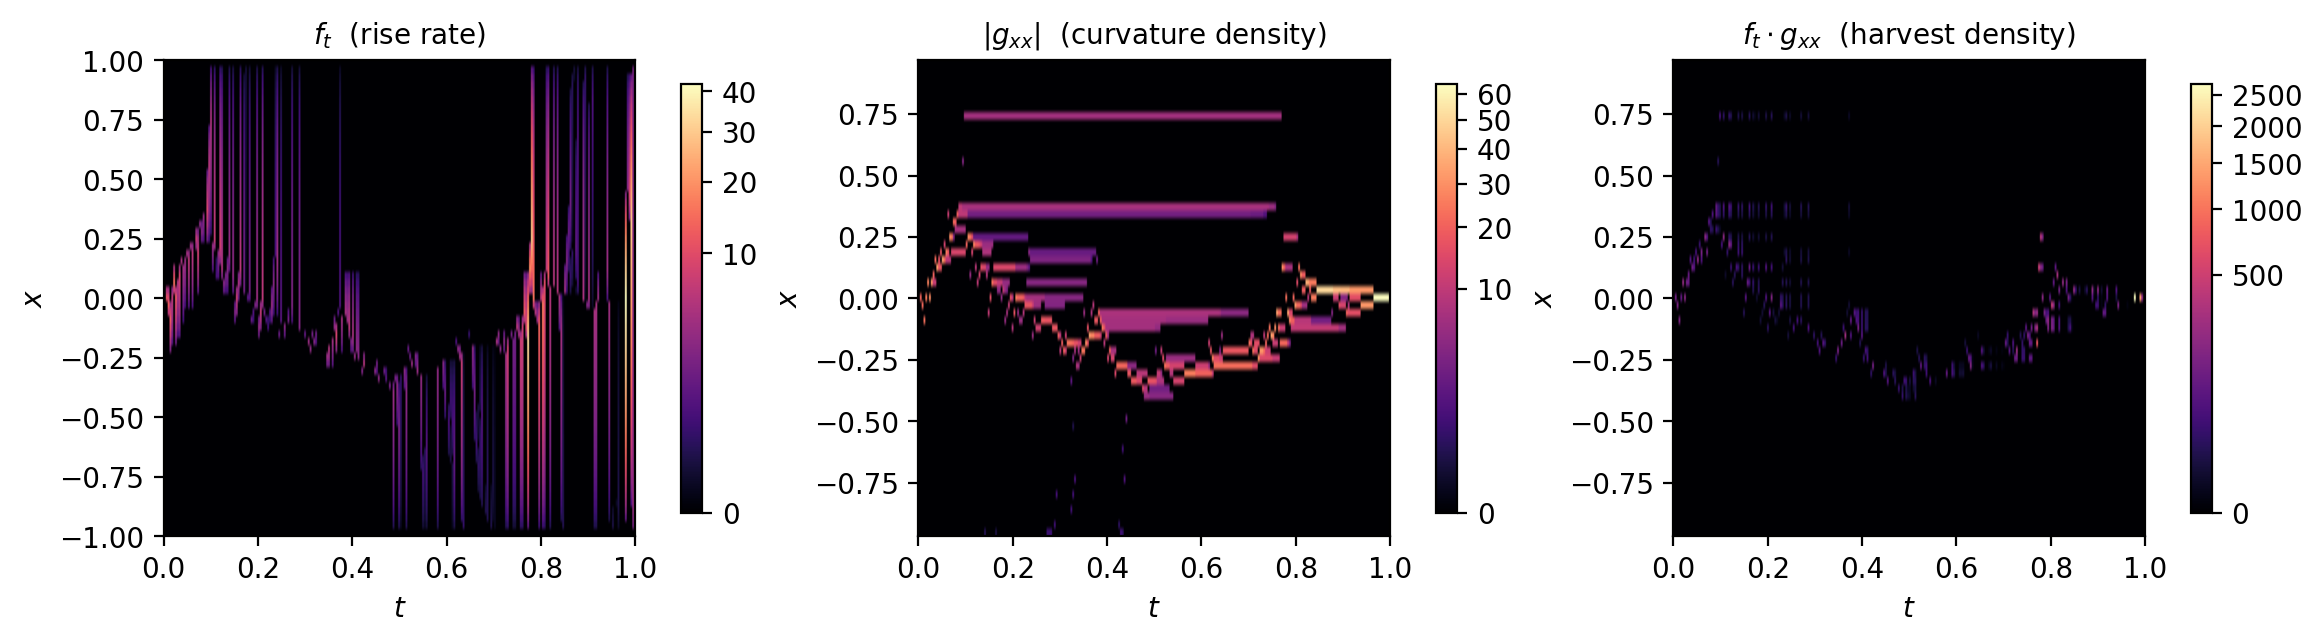
\includegraphics[width=\textwidth]{fig_melt.png}
\caption{The dynamics of the $J=3.055$ solution in the $(t,x)$ plane. Left:
the rise rate $f_t$ concentrates in tall, narrow, \emph{moving} filaments.
Center: the curvature density $|g_{xx}|$ forms a finite-width band that
drifts across the domain (the arc descending to $x\approx-0.4$ and
returning), shedding persistent sub-bands. Right: the harvest density
$f_t\,g_{xx}$ --- the integrand of \eqref{eq:J} --- is supported where the
two co-move, in branching self-similar filaments. Color scales are
power-law-compressed to make the faint fine structure visible.}
\label{fig:melt}
\end{figure}

Figure~\ref{fig:melt} shows why melting pays. The rigid tent parks its
curvature at one $x$ and can only ever harvest that column's rise budget
\eqref{eq:rise}; the accounting of Observation~\ref{obs:tent} then
telescopes to exactly $2$. The melted $g$ \emph{sweeps} its curvature band
across the domain, and every location it visits still holds its own
untapped budget $1-|x|$ --- stocked, at full depth, by the tent-shaped end
slice. Dually, $f$ melts so that its rise rate $f_t$ is a tall, narrow
spike \emph{co-moving} with $g$'s band (Figure~\ref{fig:melt}, left and
right panels), keeping the harvest dense everywhere the band goes. Same
curvature mass, far more overlap.

\section{Why the gain per octave can be constant: scaling analysis}
\label{sec:scaling}

The harvest heatmap (Figure~\ref{fig:melt}, right) shows the coarse drifting
basin carrying finer, faster sub-filaments --- the melt appears
\emph{self-similar}, one generation per dyadic octave of spatial
resolution. The measured increments (Table~\ref{tab:levels}) are
$+0.211$ and $+0.219$ per octave: constant within $4\%$. If that constancy
persists, $J\sim 2+0.215\,(k-3)\sim 0.215\log_2 N_x\to\infty$. The question
is whether it \emph{can} persist, and the answer depends delicately on
\emph{which} self-similarity is meant.

\subsection{Strict self-similarity is bounded}

Contract a feasible local structure by $x\mapsto\lambda x$,
$t\mapsto\tau t$. The Lipschitz cap forces the amplitude to contract with
the width, $f\mapsto\lambda f(x/\lambda,\,t/\tau)$. Then
\[
f_t\sim\lambda/\tau,\qquad g_{xx}\sim 1/\lambda,\qquad
\dd x\dd t\sim\lambda\tau
\qquad\Longrightarrow\qquad J_{\mathrm{local}}\sim\lambda .
\]
A cascade of strictly contracted copies therefore contributes
$\Delta J_k\sim\lambda^k$: a geometric series, bounded, \emph{regardless of
any budget considerations}. This rules out the most natural construction
--- and explains, in hindsight, why a previous constructive experiment
built precisely this way (each generation an affine-contracted copy
anchored at its parent's endpoint) found rapidly decaying gains and
concluded boundedness. That conclusion is real but applies only to the
strictly self-similar ansatz, which the present analysis shows could never
have blown up in the first place.

\subsection{Anisotropic scaling gives constant gain}
\label{sec:aniso}

Now let generation $k$ contract its band width, lifetime, and rise share
--- but \emph{not} its travel length:
\[
w_k\sim 2^{-k},\qquad s_k\sim 2^{-k},\qquad r_k\sim 2^{-k},
\qquad L_k\sim L=O(1),
\]
where $r_k$ is the rise deposited per swept location. Each budget closes:
$\sum_k r_k\le 1-|x|$ per location \eqref{eq:rise}; $\sum_k s_k\le 1$ for
the (near-disjoint) lifetime windows; and because the windows are disjoint
in time, the per-slice curvature cap \eqref{eq:mass} \emph{renews} across
generations --- each generation's band may carry mass $m_k=O(1)$.

Generation $k$ sweeps at speed $v_k=L/s_k$ and deposits rise share $r_k$
per swept location, so its rise-rate spike has height
$h_k\sim r_k v_k/w_k$ and its contributions to \eqref{eq:H} and
\eqref{eq:J} are
\begin{equation}
\label{eq:constgain}
\Delta H_k\;\sim\; h_k\,s_k\;=\;\frac{r_k\,L}{w_k}\;\sim\;
\frac{2^{-k}\cdot O(1)}{2^{-k}}\;=\;\text{const},
\qquad
\Delta J_k\;\sim\; m_k\,\frac{r_k\,L}{w_k}\;\sim\;\text{const}.
\end{equation}
Constant gain per octave, for $k\lesssim\log_2(1/w_{\min})$ octaves ---
exactly the staircase the mesh measures, and exactly the amplification
$L/w$ (spread the curvature thin, drag it far) that melting realizes
geometrically. \emph{Melting is anisotropic self-similarity:} $w$, $s$,
$r$ contract; $L$ does not.

\subsection{The obstruction: the re-arm cost}
\label{sec:rearm}

The one budget \eqref{eq:constgain} does not obviously close is
\emph{slope slack}. A fine band of depth $d_k$ and width $w_k$ needs slope
excursion $\sim d_k/w_k$ \emph{on top of} the coarse profile it rides. On
the coarse arms the Lipschitz budget is already saturated at slope
$\pm1$: zero slack. Slack exists only near the coarse basin's bottom,
where the slope passes through zero --- so generation $k{+}1$ is confined
to ride the bottom of generation $k$'s basin, and the width of that
rideable region is what generation $k$ implicitly pays to host its
successor. We call this the \emph{re-arm cost}. The dichotomy is:

\begin{quote}
$H[f]\to\infty$ (and $\sup J=\infty$) \emph{iff} the melt can keep
sharpening ($w\to0$) without the re-arm cost eating the per-octave gain
\eqref{eq:constgain}.
\end{quote}

The mesh data says the gain is \emph{not} eaten --- over two octaves. Two
octaves cannot distinguish a constant from a slowly decaying sequence, and
the measurement is expensive in exactly the wrong way: a clean octave must
refine $N_x$ \emph{and} $M_t$ together (Table~\ref{tab:levels}, levels
7--8 show what happens otherwise: the fine travelling melt-fronts are
time-unresolved and $J$ regresses), so the cost per octave grows
fourfold and the mesh is permanently capped near where it already is.

\section{A renormalization cell problem}
\label{sec:cell}

The way out of extrapolation is to make the per-generation structure
itself the object of study. Because the proposed optimum is a cascade of
rescaled generations, one generation in its own rescaled frame is a
\emph{fixed-size} problem, independent of $k$:
\[
\hat x=\frac{x-c(t)}{w_k},\qquad \hat t=\frac{t-t_k}{s_k},
\]
with $c(t)$ the band-center path. In these coordinates a generation is
specified by $O(1)$ data, and $n$ generations cost $O(n)$ --- versus
$O(4^n)$ for the global mesh.

Figure~\ref{fig:hypo} sketches the hypothetical object this construction
targets: a cascade of drifting curvature bands, each contracting in width,
lifetime and rise-share by a factor $\sim2^{-k}$ while retaining an $O(1)$
travel length, every finer generation riding the basin bottom of the
coarser one and reaping the rise budget $1-|x|$ at the fresh locations it
visits. Whether the per-generation gain $\Delta J_k$ stays constant (giving
$J\to\infty$) or decays (giving $J$ bounded) is precisely the fixed-point
question below.

\begin{figure}[ht]
\centering
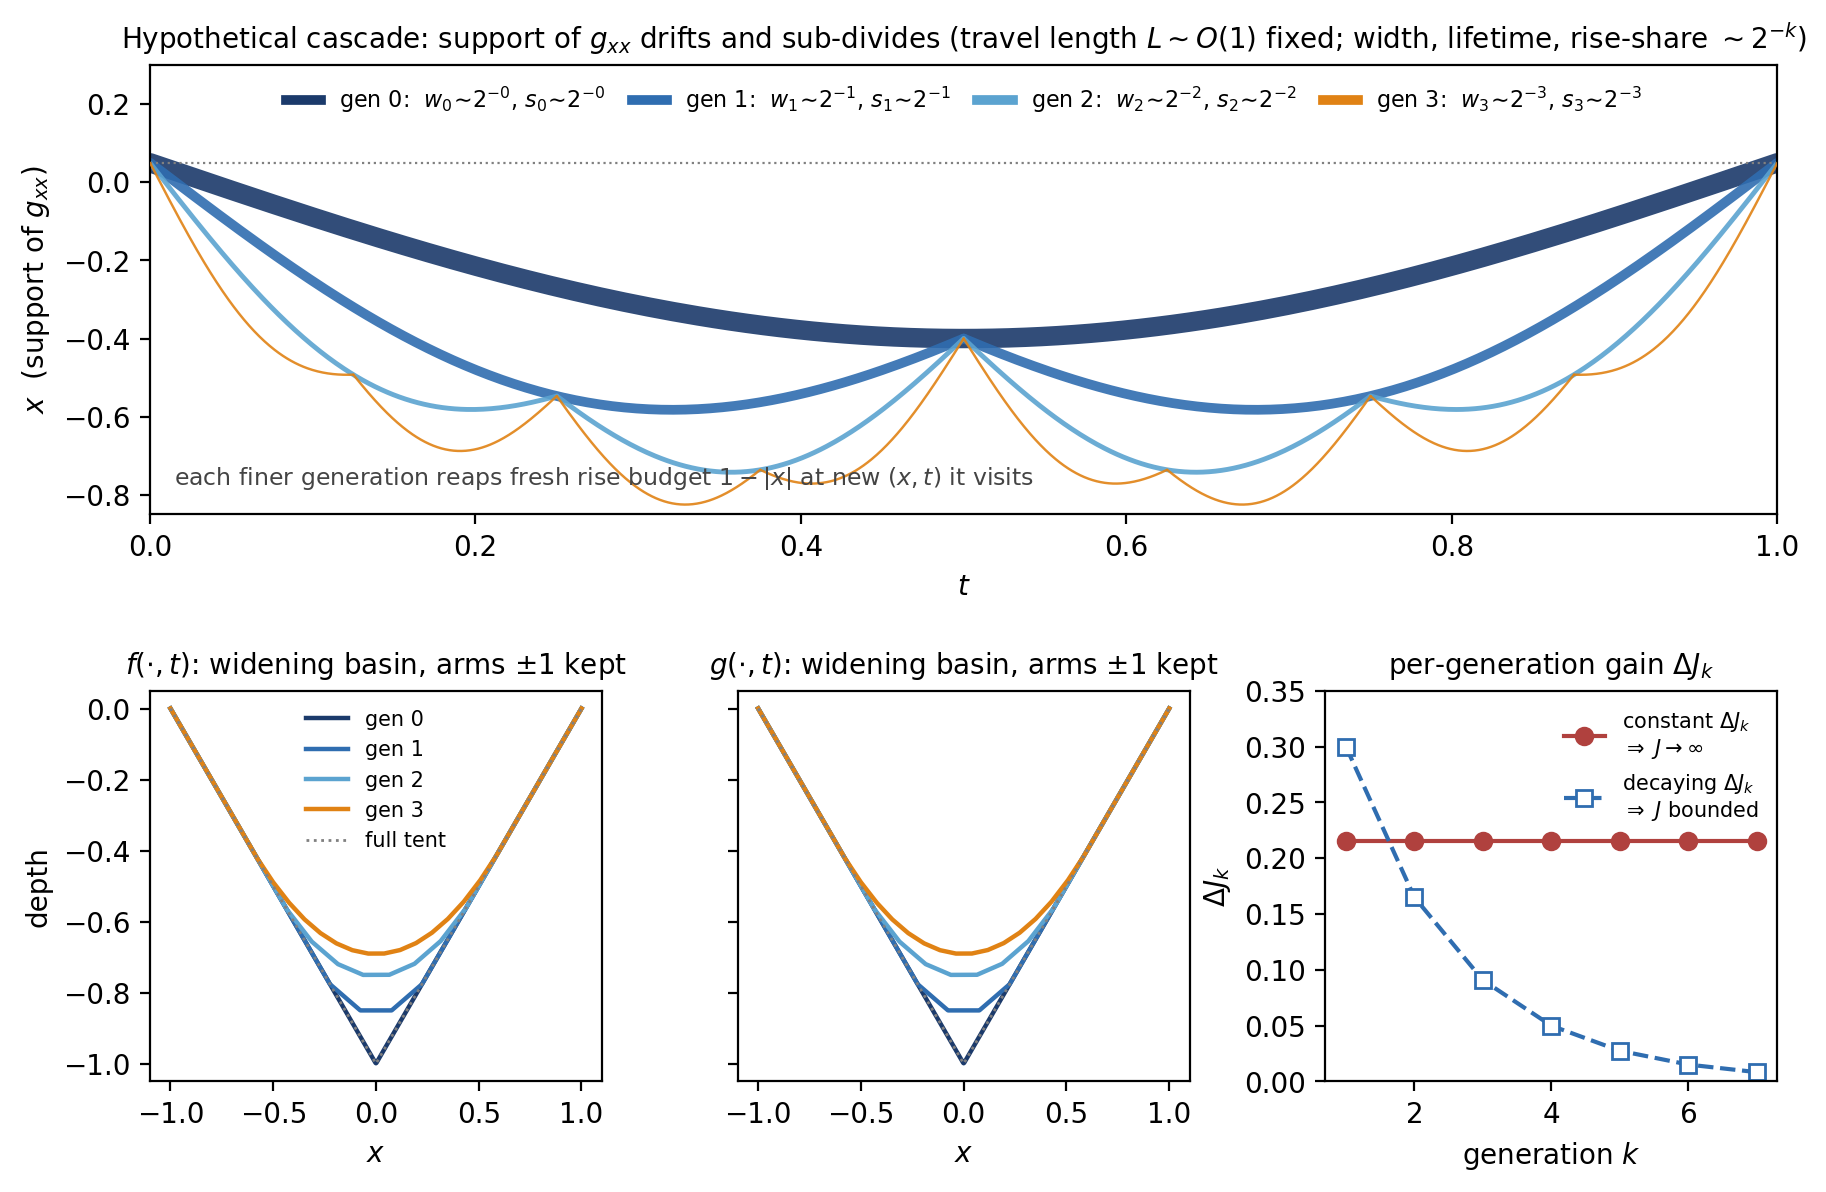
\includegraphics[width=\textwidth]{fig_hypo.png}
\caption{\emph{Hypothetical} blow-up construction (schematic, drawn by
formula --- not an optimizer output). Top: the \emph{support of $g_{xx}$}
(the location in $x$ of $g$'s curvature band, not $g$ itself) traced against
$t$; generation $0$ is a slow, wide, full-lifetime sweep, and each finer
generation halves its band width and lifetime while keeping an $O(1)$ travel
excursion, tiling its parent's window and riding its basin bottom. Bottom
left/center: the corresponding $f$ and $g$ interior
slices --- the Lipschitz-1 arms are preserved while the vertex melts into a
widening, refining basin. Bottom right: the decisive dichotomy --- constant
per-generation gain $\Delta J_k$ sums to $+\infty$ (log-growth in $N_x$);
geometrically decaying $\Delta J_k$ sums to a finite bound. The
renormalization cell is built to decide which occurs.}
\label{fig:hypo}
\end{figure}

\paragraph{The cell.} A single generation, inserted into an
\emph{environment} that summarizes everything the coarser generations left
behind: a slope-slack profile $\beta(\hat x)$ (Lipschitz budget remaining
near the host basin bottom) and a remaining-rise profile $\rho(\hat x)$
(budget \eqref{eq:rise} not yet spent). The cell's parameters are the
contraction ratios $(\lambda_w,\lambda_s)$ and the travel length $\hat L$.
Solving the cell (its feasible structure is determined by convex
programs once positions are fixed by the ansatz --- no nonconvex search,
hence no optimizer artifacts) yields two outputs: the certified gain
$\Delta\hat J(\beta,\rho;\lambda_w,\lambda_s,\hat L)$, and the
\emph{outgoing} environment $(\beta',\rho')$ the band leaves for its
successor.

\paragraph{The fixed point and the dichotomy.} Iterating the environment
map $E\mapsto E'$ and demanding self-consistency --- the incoming
environment of generation $k{+}1$ equals that of generation $k$ after
rescaling --- turns the cascade into a fixed-point problem. At a fixed
point $E^\ast$ the gain ratio $\gamma=\Delta\hat J_{k+1}/\Delta\hat J_k$
is a single well-defined number:
\begin{itemize}
\item $\gamma=1$ (a self-reproducing environment with gain bounded below):
every generation gains at least a fixed $c>0$, and by induction
$J\ge J_0+cn$ for all $n$ --- $\sup J=+\infty$ and $H[f]\to\infty$;
\item $\gamma<1$ (the environment strictly degrades and the degradation
compounds): the gains are summable, $J$ is bounded, and the proof
\emph{names the mechanism} --- the re-arm cost of
Section~\ref{sec:rearm} eating the gain at rate $\gamma$.
\end{itemize}

\paragraph{Why this can prove, not merely suggest.} A blow-up proof needs
only a lower bound and induction: (i) a \emph{gadget lemma} --- one
explicit feasible generation-insertion with $\Delta J\ge c>0$ after
paying its re-arm cost in environment $E$; (ii) a \emph{composition
lemma} --- the post-insertion state contains a rescaled copy of $E$ with
the same dimensionless data. The numerics' role is to \emph{find} the
gadget and locate the fixed point; verification is then exact, because
everything in the construction is piecewise linear with finitely many
kinks --- feasibility and the value of $\Delta J$ reduce to finite lists
of rational inequalities. The global mesh can never supply step (ii)
(its optima carry no composable structure), and the strictly
self-similar construction supplies (ii) with a gadget class that
Section~\ref{sec:scaling} shows can never satisfy (i) with constant $c$.
The anisotropic cell is the first instrument with both halves. Failing a
full proof, the $O(n)$ cost still buys a ten-octave measurement of
$\gamma$ where the mesh affords two.

\section{Honest caveats}

\begin{enumerate}
\item The constant-increment evidence rests on \emph{two} clean octaves.
The measurement is budget-sensitive in a way that mimics the signal
(time-starved refinement produces decaying gains indistinguishable from
genuine saturation --- levels 7--8), and this failure mode has recurred,
in different guises, in every numerical instrument applied to this
problem so far. Any future number must clear a resolution-convergence
gate before being believed.
\item The scaling argument of Section~\ref{sec:aniso} is an accounting of
budgets, not a construction: it shows constant gain is \emph{not excluded}
by the rise, time, and curvature budgets, while identifying the slope-slack
budget (Section~\ref{sec:rearm}) as the one that will decide. It does not
prove the anisotropic cascade is feasible at all depths.
\item The dichotomy of Section~\ref{sec:cell} is honest only if the
fixed-point search is exhaustive over its ansatz class; a $\gamma<1$
verdict is always relative to the ansatz (a richer band shape or drift
path could still blow up), whereas a $\gamma=1$ verdict with verified
gadget and composition lemmas is unconditional.
\end{enumerate}

\end{document}
